\documentclass[12pt]{article}

\usepackage[letterpaper,margin=1in]{geometry}

\usepackage{hyperref}
\usepackage{tcolorbox}

\usepackage{graphics}
\graphicspath{ {images/} }

\newcommand{\loc}[1]{
{\bf \fontfamily{pcr}\selectfont #1}
}

\newcommand{\todo}[1]{ \begin{tcolorbox} \centering  #1 \end{tcolorbox}}

\newcommand{\key}[3]{{\loc{#1}} (#2) : #3}


\title{UCLA HEDP Experimental Plasma Physics Analysis Package Documentation}
\date{\today}
\author{Peter Heuer}


\begin{document}
\emergencystretch 3em

\maketitle

\newpage

\tableofcontents

\newpage

\section{Overview}

\begin{figure}[h]
\centering
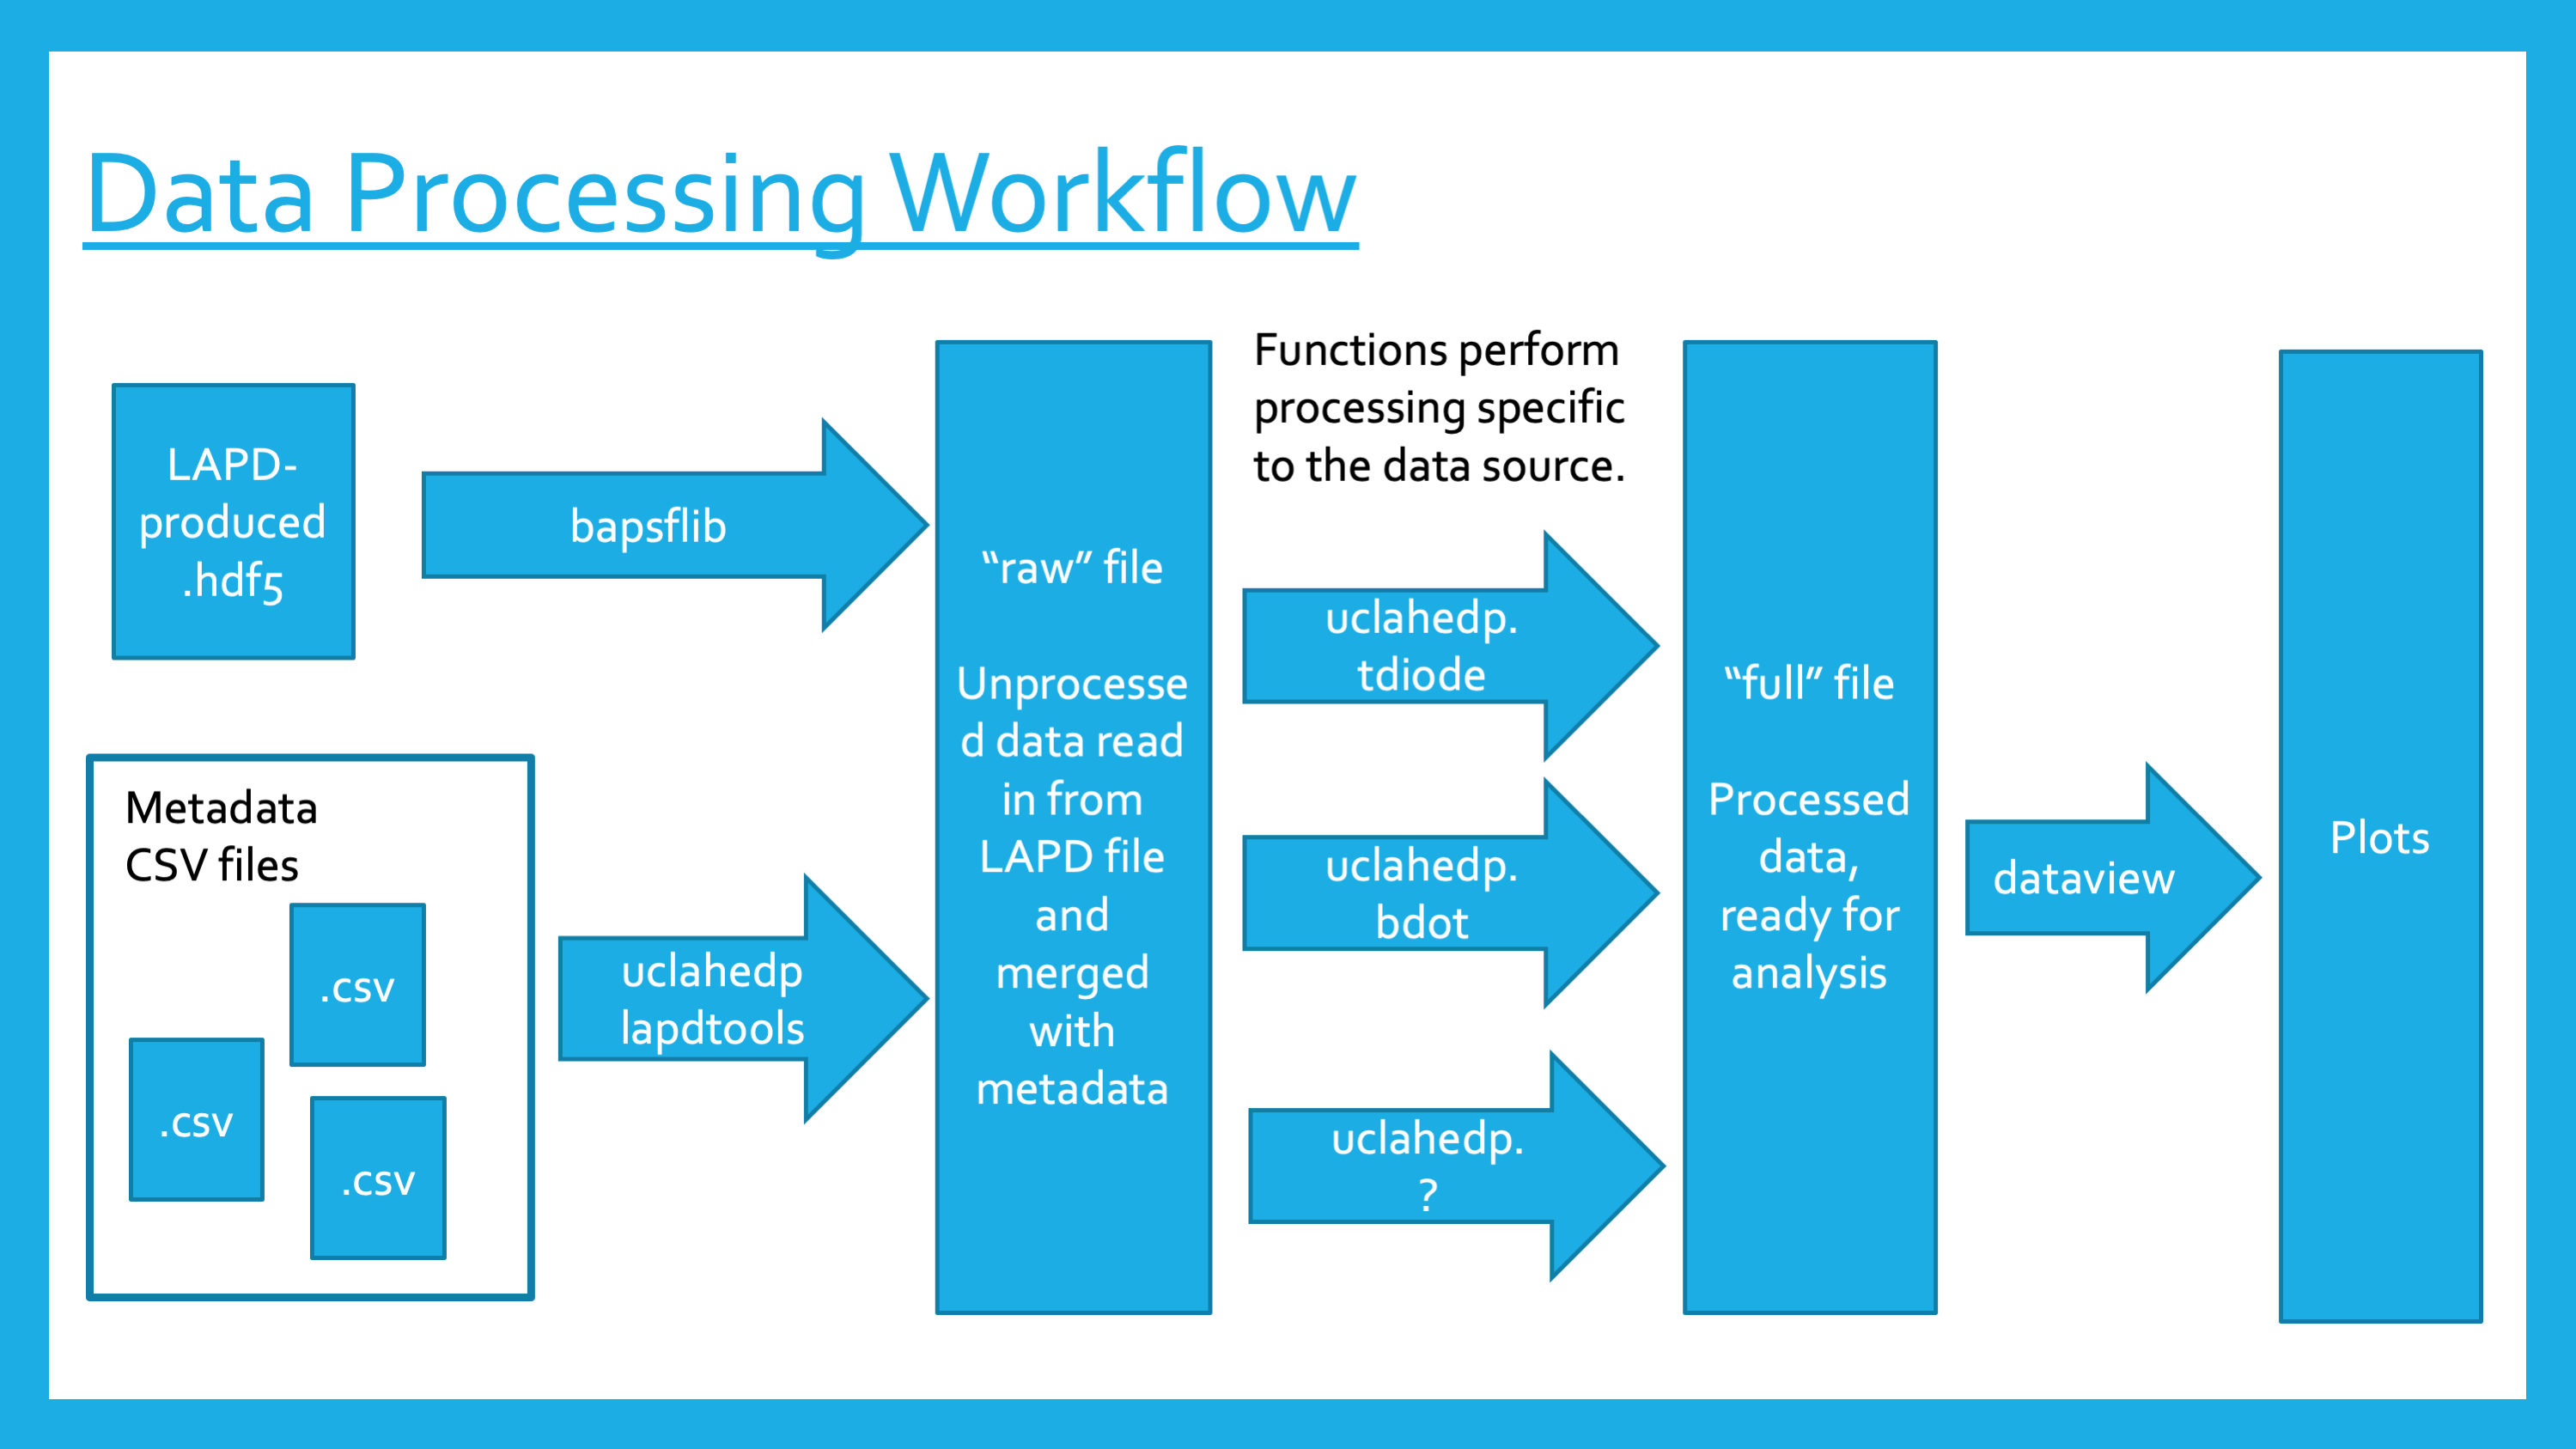
\includegraphics[width=\textwidth]{process_flow}
\caption[Processing Workflow]
{\label{process_flow} A visualization of the processing pipeline.}
\end{figure}

The UCLA HEDP package provides a pipeline for turning  raw datafiles from a number of sources into fully-processed data ready for analysis. The package also includes a toolkit of analysis routines intended to reduce code duplication for common tasks like filtering data. Throughout the pipeline all data is stored in a common format (the CDF format) which enables all data at any point to be plotted using a common plotting routine, provided by the \loc{dataview} program.

The processing pipeline takes datafiles from several sources as inputs, as well as metadata CSV files that adhere to a standard format. In the first stage of processing, these various data sources are merged with metadata and saved in a standardized format. No physics is accounted for in this stage. In the second stage, these "raw" files are transformed into "full" files. In this stage, raw voltage values are transformed into physically meaningful outputs ready for higher level analysis. The abstraction of the "raw" processing step from the "full" step allows data from a Langmuir probe (for example) hooked up to any data source to be processed by the same Langmuir probe processing routines.


\subsection{Concepts}

Throughout the pipeline (and the associated metadata CSV format), data is labeled using two important concepts:

\begin{itemize}
\item \textbf{probes}: A probe is a a string that labels a particular measurement source. A probe could have an associated position (like a bdot) or not (like a timing photodiode). A probe can correspond to any number of digitizer channels. A probe can have metadata associated with it either permanently or only for a single experimental run. 

\item \textbf{runs}: A run is a repetition of the experiment (or multiple repetitions) that belong conceptually together and are therefore stored and processed together. A run can involve multiple probes. A run can have metadata associated with it (independent of any probes). A run is represented by a run number.
\end{itemize}

\begin{figure}[h]
\centering
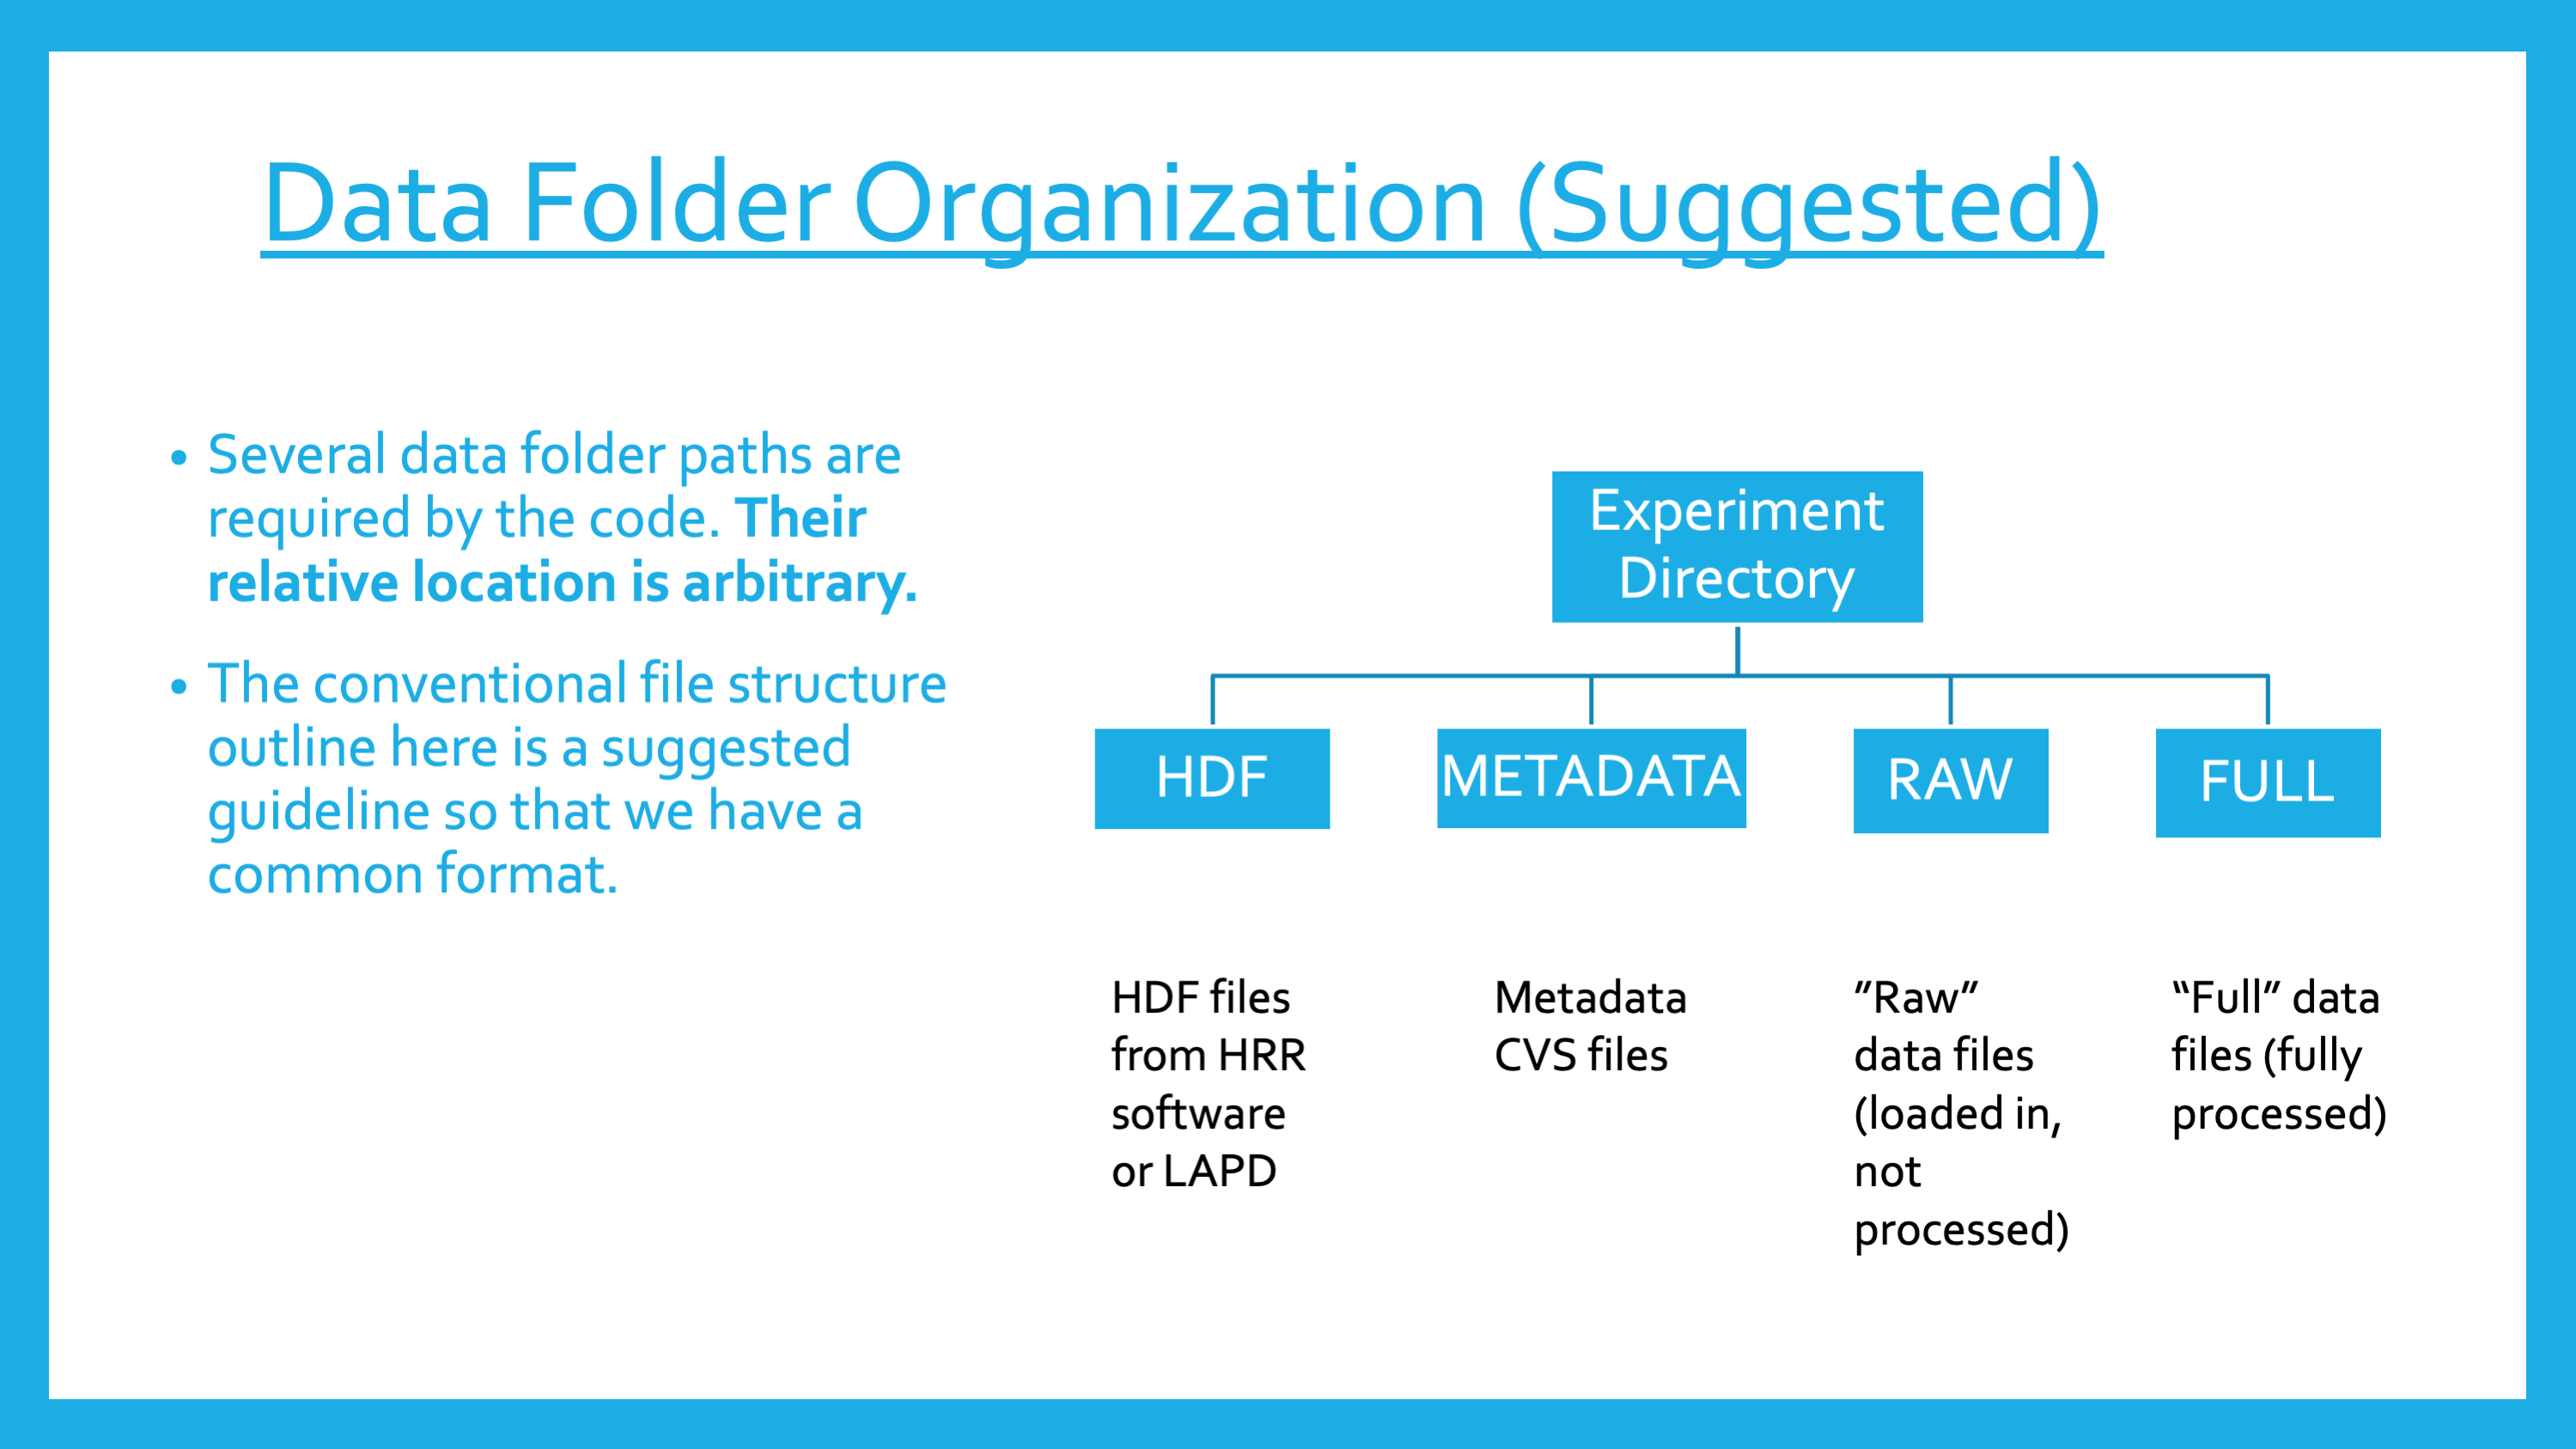
\includegraphics[width=\textwidth]{file_struct}
\caption[File Structure]
{\label{file_struct} A recommended file structure for storing data.}
\end{figure}

When storing datafiles for an experiment, it is recommended (but not strictly required) for the following system of sub-directories to be used:

\begin{itemize}

\item \textbf{METADATA}: This directory is where the package will search for any metadata CSV files. All files in this directory (and in sub-directories recursively) will be searched. 

\item \textbf{HDF}: This is where the original HDF files are stored.

\item \textbf{RAW}: This is where output of the raw or "load" processing step is stored.

\item \textbf{FULL}: This is where the the fully processed datafiles are output.

\end{itemize}

All of the routines within the package take a full filepath to specify the data to load in and write out, so the data need not be stored together (except for metadata, which must be collected in a directory so it can be searched). 



\subsection{Philosophy}

A few guiding principles that guided the design choices behind the structure of the UCLA HEDP package include:

\begin{itemize}

\item \textbf{Only original datafiles and metadata should need to be stored}.\\ Processed datafiles should be easy enough to create that they can be re-created when needed from the original datafiles and metadata. This principle saves disk space and also ensures that the data being used was processed using up-to-date metadata (as opposed to a saved processed datafile whose origins may be unclear). 

\item \textbf{When possible, data should be stored in a common format that can be easily plotted.}\\ Storing data in a common format (in this case the CDF format) enables standardized plotting routines which make it easy to check data at different stages of analysis. 

\item \textbf{Minimize the amount of data in RAM at any time}. Any computer should be able to process any dataset, given sufficient time. Programs should take advantage of the HDF file format to only load parts of the data in memory during processing so that even laptop computers can process 100 GB datafiles.

\item \textbf{Reduce code duplication through standardization}. A bdot is the same probe whether it is used in LAPD or in the Phoenix lab, and it should therefore be processed using the same bdot routines.

\end{itemize}


\section{The Common Data Format (CDF)\label{cdf}}

\begin{figure}[h]
\centering
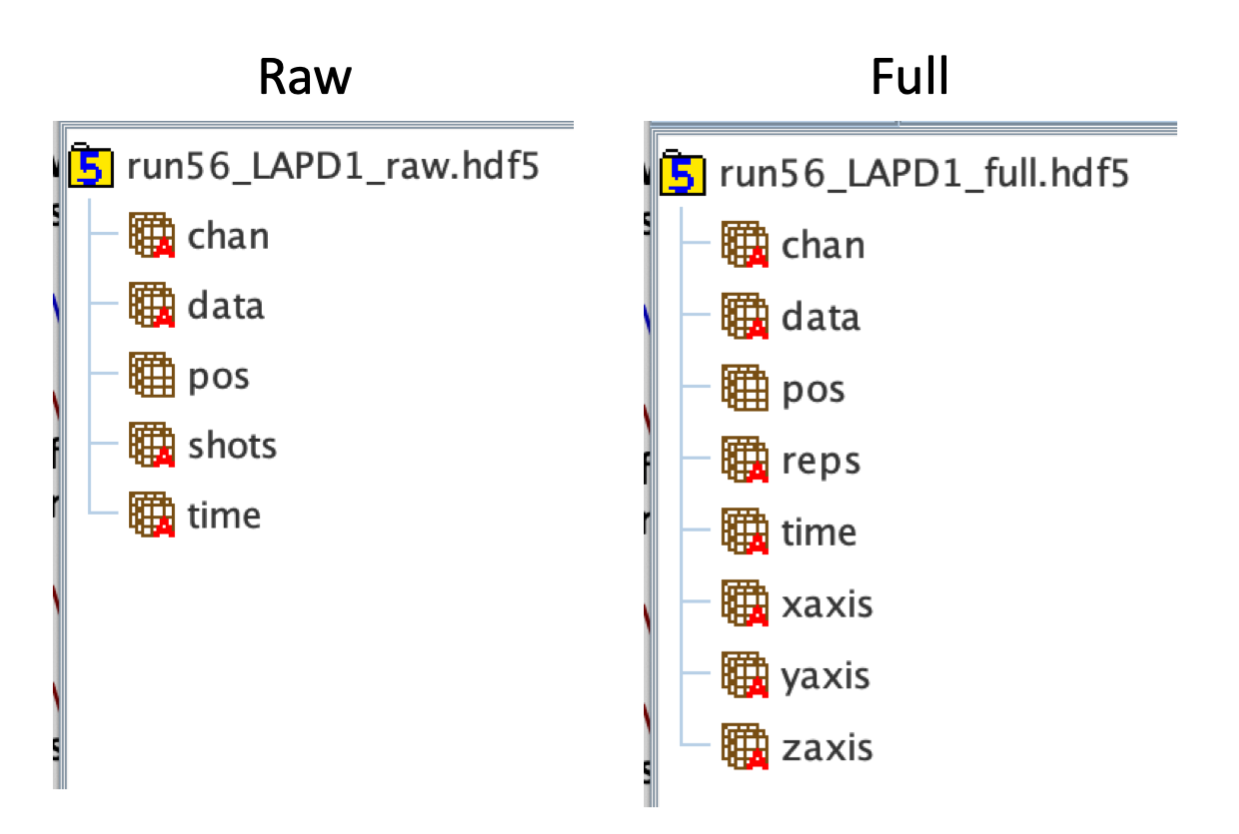
\includegraphics[width=0.7\textwidth]{hdf5_struct}
\caption[Example of CDF HDF5 Files]
{\label{hdf5_struct} Example structures of a raw and a full HDF5 file that conform to the CDF.}
\end{figure}


\subsection{Requirements}

The UCLA HEDP package is designed around a standardized structured data format, hereafter referred to as common data format or CDF. A CDF object is an HDF file that conforms to a standard structure as defined in the function \loc{tools.dataset.validDataset}. In particular, each CDF file must contain

\begin{itemize}

\item A CDF object is a group in an HDF file. It may be the root group, or multiple CDF objects may be housed within a HDF file as separate groups.

\item A dataset called "data" with $n$ dimensions. This array must have an attribute "dimensions" which holds a string array of list $n$ which provides a name for each dimension in the dataset (by convention, all lowercase). A second attribute "unit" defines the units of the data in this array as a string that can by interpreted by the \loc{astropy.units} string-to-unit parser. 

\todo{In the future this could be generalized so that the CDF object could contain multiple data arrays with different names (but all with the same shape and the same axes). This would be conducive to datasets such as density and electron temperature planes from Langmuir measurements which share a set of axes and belong conceptually together. In this case, a new attribute array should be added to the parent group listing the names of all of the data arrays. }

\item For each entry in the "dimensions" attribute there must exist a dataset with the same name which contains the axis values for that dimension. This dataset must also include a mandatory "unit" attribute as defined above.

\item Other attributes (commonly including metadata) are included as attributes of the root group in the HDF file. These entries should be tuples of the form (value, unit) where unit is a unit string as described in the previous points.

\end{itemize}

This format was designed to contain all of the information necessary to make plots of the dataset.

\todo{
One notable exception to the CDF format is probe position information which is saved in an additional array called "pos" with dimensions [shot num, 3] and has no attributes. Other similar non-standard arrays include t0ind and badshots in timing diode files. These "special" files that contain these additional required array should be considered subclasses of the CDF format - they inherit all of the normal requirements but also require these additional arrays.
}

\subsection{Conventions}
\begin{itemize}
\item The convention [shots, time, channels] is commonly used for raw shot-ordered datasets.
\item The convention [time, xaxis, yaxis, zaxis, repetition channel] is commonly used for processed volumetric datasets. 
\end{itemize}

These conventions are chosen to allow easy plotting of subsets of an array. For example, if a dataset has dimensions B = [time, xaxis, yaxis, zaxis, repetition channel]. then it is easy to extract a time trace for a particular position, repetition, and channel B[t] = B[:, x, y, z, r, c] (where x,y,z,r,c represent fixed values for the other axes) or an XY plane B[x,y] = [t, :, :, z, r, c]. 

\subsection{Considerations for Large Datasets}

Large datasets are not stored on consecutive sections of computer memory but are rather broken into "chunks" that are stored separately. Accessing data spread across multiple chunks is much more computationally costly than accessing the same amount of data from a single chunk. The HDF format and the \loc{h5py} package allow control over how a dataset is broken into chunks in order to maximize efficiency. Where possible, the UCLA HEDP package attempts to chunk datasets in a way that minimizes read times for common operations. For example, a dataset containing time arrays at a variety of spatial locations may chose to chunk the time axis together, anticipating that time traces may be accessed more often than large spatial volumes.


\section{The CSV Metadata Format\label{csv_format}}

\subsection{CSV File Header Format}

Metadata is recorded in CSV files in a standard format, and many column header names may be required by different routines in the analysis pipeline:

Across all metadata files the following header format is followed for the top three rows
\begin{enumerate}
\item Machine-readable keywords, eg. "probe", that will become dictionary keys.
\item Unit string, or blank for dimensionless units, eg. "mm2"
\item Human-readable title or note, eg. "Bdot Area". This row is not used by the program but improves readability of the CSV file.
\end{enumerate}

\subsection{The Four Types of Metadata Files}
Metadata files are sorted into four types automatically based on whether the csv file includes the "run" or "probe" keywords (Table~\ref{csv_types}). This system allows information that does not change throughout the experiment for either one or all probes to not be repeated unnecessarily, which keeps the metadata files managable and reduces errors.

\begin{table}[]
\begin{tabular}{p{1cm}p{2cm}p{2cm}p{6cm}}
Type                                 & Has "run" key? & Has "probe" key? & Explanation                                                                          \\ \hline
\multicolumn{1}{c|}{Experiment Type} & No             & No               & Data that pertains to the whole experiment, eg. experiment name, vacuum chamber used \\
\multicolumn{1}{c|}{Run Type}        & Yes            & No               & Data that pertains to a given run number, eg. background field, fill pressure        \\
\multicolumn{1}{c|}{Probe Type}      & No             & Yes              & Data about a particular probe for the whole experiment, eg. calibration constants    \\
\multicolumn{1}{c|}{Run-Probe Type}  & Yes            & Yes              & Data about a probe on a particular run, eg. positon or attenuation                  
\end{tabular}
\caption{Types of CSV spreadsheets as defined by the presence of the "run" and/or "probe" keywords.\label{csv_types}}
\end{table}

A raw file for a particular probe and run will have the following metadata attached from these files:

\begin{itemize}
\item All metadata from all experiment type metadata files.

\item All metadata from all run type metadata files that match the run number.

\item All metadata from all probe type metadata files that match the probe name.

\item All metadata from all run-probe type metadata files that match BOTH the run and the probe.
\end{itemize}


\todo{Tip: Non-integer run numbers can be used to label multiple sub-runs with metadata from the main run. For example, if multiple movies are captured using a camera during run 32, which is a long probe plane, the camera runs could be labeled 32.1, 32.2 etc. and will automatically inherit the run-type metadata from run 32.}



\section{Structure of the Package}
The UCLA HEDP package is separated into several sub-packages (folders within the package) that group similar routines. The logic of these groupings, and a brief explanation of the contents of each sub-package, is provided in the following sections.


\subsection{\loc{tools}}

The \loc{tools} package contains a variety of miscellaneous functions, many of which are used widely throughout other routines.
\subsubsection{\loc{csv.py}}

The primary purpose of \loc{csv.py} is to process a directory of comma-separated value (CSV) files in a file directory containing metadata about an experiment (see Sec.~\ref{csv_format}).  A list of CSV files in a directory is created using \loc{csv.getCSVList} and then those files are read into a python OrderedDictionary object by \loc{csv.opencsv}. This package is commonly accessed from other routines through the function \loc{csv.getAllAttrs}, which returns the metadata from across all files that pertains to a particular probe and run number. Functions \loc{csv.getProbeList} and \loc{csv.getRunList} provide lists of all valid probes and runs from an experiment, which are useful when creating loops to process data.


\subsubsection{\loc{dataset.py}}

This file contains a function that tests whether an HDF group conforms with the CDF (as described in Sec.~\ref{cdf}), which is \loc{dataset.validDataset}. Another helper function \loc{createDataset} can be used to create new datasets from a group of arrays.

The remainder of this file contains functions that were intended to perform operations over large datasets in an efficient way. The function \loc{dataset.chunked\_array\_op} was intended to provide an easy way to perform operations like thinning and averaging large datasets without forcing the user to manually chunk the data. However, this scheme turned out to be too time intensive because data operations are applied one-by-one. At this time, the most efficient way to process a large dataset is still to write a custom program that performs all operations in a single pass through the file (a process which is difficult to generalize).

\subsubsection{\loc{hdf.py}}

This file contains programs for interfacing with HDF files. In particular, \loc{hdf.writeAttrs}, \loc{hdf.readAttrs}, and \loc{hdf.copyAttrs} are the preferred way to interact with attributes because they correctly translate strings to unicode and handle the (value,unit) format used in the CDF. This file also contains the \loc{hdf.hdfPath} object which is provides a convenient way to pass both a filename and a HDF group path as one object. This was created with the idea of eventually supporting HDF files with multiple CDF objects within them (as separate groups).

\subsubsection{\loc{math.py}}

This file contains mathematical functions used throughout the package. In practice most routines necessary are available in \loc{numpy} or other packages, so the only function here is a discrete curl algorithm.

\subsubsection{\loc{pos.py}}

This file contains routines for creating grids for volumetric measurements. The functions are generally called through the high-level function \loc{pos.grid}, which takes a list of positions (along with some required attributes) and outputs a list of axes as and an array for placing shots into a grid. Two steps are necessary for this process: the creation of axes and the placement of points on those axes. Two methods exist for carrying out these operations, dubbed "strict" and "fuzzy" gridding. Which of these methods is applied is controlled by keywords.

Under strict axes, axes are created \textit{a priori} based on metadata in the attributes dictionary, while under fuzzy axes axes are inferred from the provided position array. Similarly, under strict gridding shots are assigned to positions in the grid based on an \textit{a priori} assumption about the movement of the probe (and metadata), whereas under fuzzy gridding positions are discritized (to within the grid precision) and placed at the grid cell that most closely matches the probes actual location. These methods can be mixed, eg. strict axes can be used with fuzzy gridding. 

In general, fuzzy axes and gridding are more desirable. These ensure that the true location of the probes is used (a probe may not actually move to a location if it is physically unable to do so, which is not reflected in strict gridding). Fuzzy gridding also easily supports complicated probe paths and could easily be upgraded to support non-cartesian grids. Strict axes and gridding should be viewed as a backup for datasets on which fuzzy gridding fails for some reason.

\todo{Modification of these routines to support grids in polar coordinates should be a relatively high priority in future in order to support "fan" grid patterns on radial probe drives like those on the LAPD.}


\subsubsection{\loc{util.py}}

This file contains several convenience functions, the most widely used of which is the \loc{util.timeRemaining} object which is used to create progress timers for various operations throughout the package.

\subsection{\loc{load}}

The \loc{load} subpackage provides routines for transforming data from several sources into the standard CDF format. Once data is in this format, it can be processed by other routines in the package without regard to its origin.

Load routines also take a csv directory and merge the relevant attributes (based on the selected probe and run) with the dataset. This metadata is then attached to the HDF file, so changing the metadata necessitates re-processing the data from the beginning starting with the load command. This choice was made intentionally to ensure that consistent metadata is used throughout the processing of a dataset.

\subsubsection{\loc{lapd.py}}

These programs load data from HDF files output by the LAPD DAQ system using the \loc{bapsflib} package. The routine can currently import position information from three probe drives: the XY drive, the XYZ drive, and the XY drive (6K Compumotor). 

\todo{Originally only the 6K Compumotor was supported by \loc{bapsflib}, and so the other drives were handled manually. Support for other drives has now been added to \loc{bapsflib}, so these routines could be updated to use that functionality.}

\subsubsection{\loc{hrr.py}}

These programs load data from HDF files output by the Phoenix Terminal's High Repetition Rate experiment software. 

\subsubsection{\loc{imgdir.py}}

This program loads a directory of images, commonly used to import frames from a camera. Images are loaded in an order determined by their filenames using a natural sorting algorithm.


\subsubsection{\loc{ascii.py}}

This program loads data from an ASCII file, intended for creating CDF objects out of simulation output or output from instruments like oscilloscopes. 

\todo{This program may not be finished, but would be a useful tool. An additional desirable feature would be the ability to load whole directories of ASCII files and combine them intelligently into one CDF.}


\subsection{\loc{process}}

The \loc{process} subpackage is the core of the UCLA HEDP package, containing routines that transform raw data into processed data ready for analysis. Each file described below processes data for a particular diagnostic or instrument. The example script \loc{process.process.py} shows how all of these routines (along with those throughout the package) can be used to turn raw datasets and metadata files into processed output files.

\subsubsection{\loc{bdot.py}}

The primary function in this file is \loc{bdot.bdotRawToFull} which processes raw magnetic flux probe measurements into measurements of the vector magnetic field. Several of the keywords in this function merit some explanation

\begin{itemize}
\item \loc{replace\_badshots} If this keyword is set, shots marked as bad by the tdiode routine will be copied over by the nearest good shot.

\item \loc{offset\_range} gives the range (in indices) over which the voltage offset of the signal will be calculated. This should done at a time when the real signal is nominally zero. 

\item \loc{offset\_rel\_t0} allows the user to set values in the previous variable as being relative to to the laser firing. A common configuration is for the start of the offset range to be fixed at zero, but the end to be set to be just before the laser pulse. In this case the user may set \loc{offset\_range} = (0, -50) while \loc{offset\_rel\_t0} = (False, True). 
\end{itemize}

This file also contains two functions \loc{bdot.fullToCurrent} and \loc{fbdot.ullToBmag} which take a fully processed bdot signal and calculate either the current (using the curl and neglecting the displacement current in Ampere's law) or the magnitude of B. 

The file also contains the \loc{bdot.calibrateProbe} function which performs fits to calibration data recorded in a CSV file by a network analyzer. This program assumes a standard Helmholtz coil configuration is used to calibrate the probe. 

\todo{The current \loc{bdot.calibrateProbe} function can only handle CSV files, while the network analyzer used at UCLA for this purpose outputs \loc{.dat} files. Reading these files directly should be possible, and adding that functionality to this function would be very helpful.}

\subsubsection{\loc{tdiode.py}}

This program takes in data from a timing diode (typically a photodiode positioned in the leak of a laser mirror that shows the laser pulse) and determines the index corresponding to the rise of the pulse (corresponding to t0). The program also identifies bad shots (no laser) by comparing the maximum of the pulse to the noise level. 


\subsubsection{\loc{langmuir.py}}

This file contains several programs for processing Langmuir probe measurements. \loc{langmuir.isatRawToFull} processes ion saturation current measurements and is relatively straight forward. \loc{langmuir.vsweepLangmuirRawToFull} processes swept Langmuir probe measurements and is considerably more complicated. The swept Langmuir probe routine makes use of several subroutines

\begin{itemize}

\item \loc{langmuir.find\_sweeps} takes a time array and a voltage trace of the ramp voltage and identifies the time ranges corresponding to each ramp. By default the swept Langmuir analysis routine will attempt to fit ever ramp (although many at lower densities may fail). 

\item \loc{langmuir.vsweep\_fit} takes a Langmuir IV curve (voltage and current traces) and fits the electron saturation and transition regions with a linear fit and an exponential fit respectively. The program attempts to intelligently determine the boundaries for these regions, but they may also be adjusted by the user. This function is designed to recognize failed fits, which are commonly caused when a probe moves into a region of lower density. These failed fits are intended to cause errors which results in the value \loc{fail\_val} being output in the parameters so these datapoints can be easily ignored in analysis.

\todo{Some rudimentary error analysis is in place for this function: in principle it should be possible to transform the covariences from the curve fits into error bars on the output quantities like density and electron temperature. In practice propagating the the errors from both fits through the formulas is non-trivial, but this would be a great project to finish in the future.}

\end{itemize}


\subsubsection{\loc{interferometer.py}}

This file contains a simple routine for computing the phase shift measured by an interferometer from a hetrodyne interferometer given the signal and the reference signal. 

\todo{The full calculation of the density from the phase shift has not yet been implemented.}

\subsubsection{\loc{imgseq.py}}

This file contains a function that transforms a CDF file created from an image directory corresponding to a sequence of images and creates appropriate physically meaningful axes for it. Attributes can be set in the metadata to change the scale of the pixels in physical units, set an origin, and create a time vector. 

\subsubsection{\loc{scope.py}}
This program is a dummy processing routine that does nothing to the data other than apply a timing diode correction. The intended use-case is for quick analysis during an experiment of instruments that are not otherwise handled by the UCLA HEDP package.

\subsubsection{\loc{process.py}}
This script is an example/template script for running all of the analysis programs in the UCLA HEDP package. The program \loc{process.process} takes runs the full sequence of analysis steps on a probe for a particular run. A raw file is created using the appropriate load function, then the appropriate final processing routine is applied.

\loc{process.processMany} runs this program in a loop over a set of runs and probes provided by the user. Combinations of runs and probes that do not apply are ignored. This allows the user to set up a large list of runs and probes (potentially an entire experiment) to run unattended.

\todo{This file should really live in the examples folder, since it's really just an example of a processing script.}





\subsection{\loc{analyze}}

The \loc{analyze} subpackage contains useful routines for data analysis. 

\subsubsection{\loc{filter.py}}
This file contains several frequency filtering tools that can be used for either temporal or spatial frequency filtering. \loc{filter.fftFilter} is a Fourier-filter than provides a bandpass (or band-block) filter on a 1D trace. \loc{filter.lowpassFilter2D} is a lowpass filter intended for spatially filtering 2D planes prior to calculating the curl in order to calculate the current.



\subsubsection{\loc{polarization.py}}

This file contains functions for analyzing the polarization of a signal based on a vector time trace either using a polarization decomposition algorithm or by creating a hodograph.

\subsubsection{\loc{spectral.spectrogram.py}}

This function implements a moving-window Fourier transform algorithm to generate a spectrogram. 

\subsubsection{\loc{thomson.thomson\_scattering.py}}

This file contains a number of routines for the prediction of Thomson scattering spectra. \loc{thomson\_scattering.spectrum} calculates the spectral density function in a variety of regimes given a description of the ion and electron distributions (assuming Maxwellians). \loc{thomson\_scattering.signal\_estimate} estimates the total number of scattered photons for use in estimating the signal-to-noise ration for a given configuration.

This program was developed prior to the implementation of \loc{diagnostics.thomson} in PlasmaPy: the implementation there is better vetted and you are encouraged to use that instead.


\subsection{\loc{user}}

Any user of the package is invited to add a folder to this section which holds code they have written that either uses the package or complements it.


\subsection{\loc{dataview}\label{dataview}}

The \loc{dataview} program is technically a separate program from UCLA HEDP (housed in a different repository) so that it can be installed without as many requirements. \loc{dataview} can visualize any CDF object. One of the benefits of using a consistent data format is that \loc{dataview} can therefore be used to look at data saved at any point during the analysis pipeline.

\appendix 

\section{Metadata CSV Key Dictionary}
This appendix defines a number of dictionary keys.
\subsection{Experiment Data}

No standard keys exist for this type of file yet

\subsection{Run-Type} 

\begin{itemize}
\item \key{datafile}{str}{Datafile name. "datafile".hdf5 should be the datafile for each "datafile" in this column.}
\end{itemize}

\subsection{Probe-Type}

\begin{itemize}
\item \key{probe\_type}{str}{Specifies the probe type, used to decide which analysis routines to run. Example: "bdot", "tdiode".}
\end{itemize}

\subsubsection{Probe-Type: Bdots Probes}

\begin{itemize}
\item \key{area}{float}{Area of the probe tip (used when calculating isat density)}

\end{itemize}

\subsubsection{Probe-Type: Langmuir Probes}

\begin{itemize}
\item \key{nturns}{int}{Number of bdot turns (assume to be the same for all axes).}
\item \key{\{xyz\}area}{float}{Area of the probe tip from calibration.}
\item \key{\{xyz\}tau}{float}{High-frequency calibration constant for each axis.}
\end{itemize}

\subsection{Run-Probe Type}

\begin{itemize}
\item \key{\{xyz\}pol}{1 or -1}{This factor is multiplied by the data that is read in to potentially reverse it if a probe was in upside down.}
\item \key{gain}{float}{Amplifier gain prior to the digitizer.}
\end{itemize}

\subsubsection{Run-Probe Type: LAPD Digitizer}

\begin{itemize}
\item \key{digitizer}{str}{Name of the digitizer used. Example "SIS crate".}
\item \key{adc}{str}{Name of the analog-to-digital converter used. Example "SIS 3305", "SIS 3302".}
\item \key{brd\{i\}}{int}{Digitizer board used, where \{i\} is the number of the channel. There should be one of these columns for each channel.}
\item \key{chan\{i\}}{int}{Channel on the digitizer used, where \{i\} is the number of the channel. There should be a corresponding "brd\{i\}" for each one.}
\end{itemize}

\subsubsection{Run-Probe Type: HRR Digitizer}
\begin{itemize}
\item \key{resource\{i\}}{int}{Resource number for each channel \{i\}.}
\item \key{chan\{i\}}{int}{Channel number. The number of these columns should match the number of resource columns.}
\end{itemize}

\subsubsection{Run-Probe Type: Probes with Position Information}

\begin{itemize}
\item \key{probe\_origin\_\{xyz\}}{float}{Position of the probe origin relative to the experiment coordinate system. These will be added to all the probe positions.}

\item \key{\{xyz\}pos}{float}{Position of the probe. Overridden by motor drive information if a probe is being scanned. These positions are relative to the probe origin.}

\item \key{roll}{float}{Angle, in degrees, that the probe was rotate about its central (x) axis. This is included during the rotation correction phase, and can be used to correct a probe that was misaligned.}

\item \key{rot\_center\_\{xyz\}}{float}{Required only for probes that rotate on a ball valve (like the LAPD probe drives). This specifies the center position of the ball valve, for use in angle corrections.}

\item \key{ax\_pol\_\{xyz\}}{1 or -1}{Direction of the motion axis relative to the experiment coordinate system. Set to -1 if they are anti-parallel. If this keyword is not included, a value of 1 is assumed by default. Currently motion axes at an angle to the experiment coordinate system are not supported (but theoretically could be added...)}

\end{itemize}

\subsubsection{Run-Probe Type: Probes Using LAPD Motor Drives}

\begin{itemize}
\item \key{motion\_controller}{str}{Which LAPD drive was associated with the probe. Example "6K Compumotor", "NI\_XYZ".}

\item \key{motion\_receptacle}{int}{Which instance of that motor drive was used? Starts at 1. For example, 6K Compumotor can control four XY drives, labeled 1,2,3,4".}

\end{itemize}


\subsubsection{Run-Probe Type: Probes Using HRR-Controlled Motor Drives}

\begin{itemize}
\item \key{\{xyz\}pos\_resource}{int}{Resource number for each channel of the probe drive.}
\item \key{\{xyz\}pos\_chan}{int}{Channel number for each channel of the probe drive.}
\end{itemize}

\subsubsection{Run-Probe Type: Bdot Probes}

\begin{itemize}
\item \key{\{xyz\}atten}{float}{Attenuation on each axis of the probe. Required to be in dB currently}
\end{itemize}

\subsubsection{Run-Probe Type: Langmuir Probes}

\begin{itemize}
\item \key{atten}{float}{Attenuation on the digitizer. Required to be in dB currently}

\item \key{ramp\_atten}{float}{Attenuation for ramp, only required for vsweep.}

\item \key{ramp\_gain}{float}{Gain on ramp signal: only required for vsweep. Regular "gain" keyword is used for the other signal channel.}

\item \key{sweep\_type}{str}{Currently "langmuir\_isat" or "langmuir\_vsweep" are used. This keyword is just useful for deciding which type of analysis routine to call on this dataset.}

\item \key{resistor}{float}{Measurement resistor for vsweep runs.}

\item \key{bias}{float}{Probe bias for isat runs.}

\end{itemize}


\end{document}